\documentclass{article}
\usepackage{graphicx}
\usepackage{lipsum}
\usepackage[T2A]{fontenc}
\usepackage[utf8]{inputenc}

\graphicspath{ {../Images/} }

\begin{document}
\begin{titlepage}
    \begin{center}
    $\newline$
    \vspace{3.3cm}
    
    {\LARGE\textbf{Лабораторна робота №1\\"Реалізація алгоритмів побайтного перетворення інформації"}}
    \vspace{10cm}
    \begin{flushright}
        \textbf{Роботу виконав:}\\Климентьєв Максим \\3-го курсу\\групи ФІ-21
    \end{flushright}
    \end{center}
\end{titlepage}
\newpage

\tableofcontents 
\section{Опис}
\textbf{RLE} --- простий алгоритм стиснення даних, який оперує серіями даних, тобто послідовностями, в яких один і той же символ зустрічається кілька разів поспіль. При кодуванні рядок однакових символів, що становлять серію, замінюється рядком, який містить сам повторюваний символ і кількість його повторів. 
\section{Особливості}
\textbf{Перенести файл на екзешник} --- і можна з ним як завгодно взаємодіяти.

\section{Кодування}
    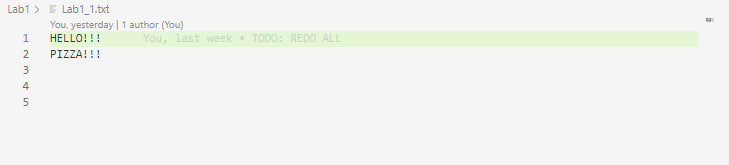
\includegraphics{Text.jpg}
    \newline
    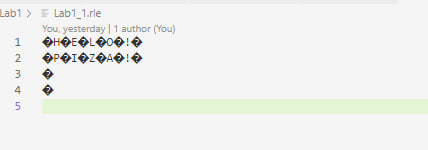
\includegraphics{Coded.jpg}

\section{Декодування}
    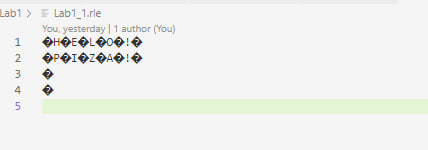
\includegraphics{Coded.jpg}
    \newline
    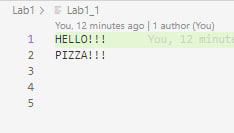
\includegraphics{Decoded.jpg}

\section{Декодування спотворених даних}
    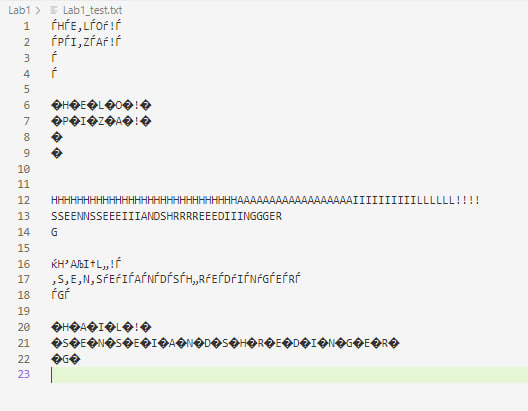
\includegraphics{Coded_Corrupt.jpg}
    \newline
    Декодер намагається декодувати і декодує усе, що в нього вийшло
    \newline
    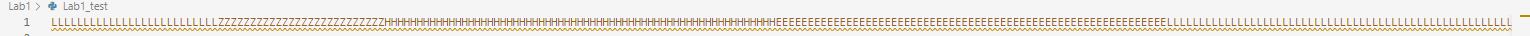
\includegraphics{Decoded_Corrupt.png}

\end{document}